\begin{figure}[!ht]
\begin{center}
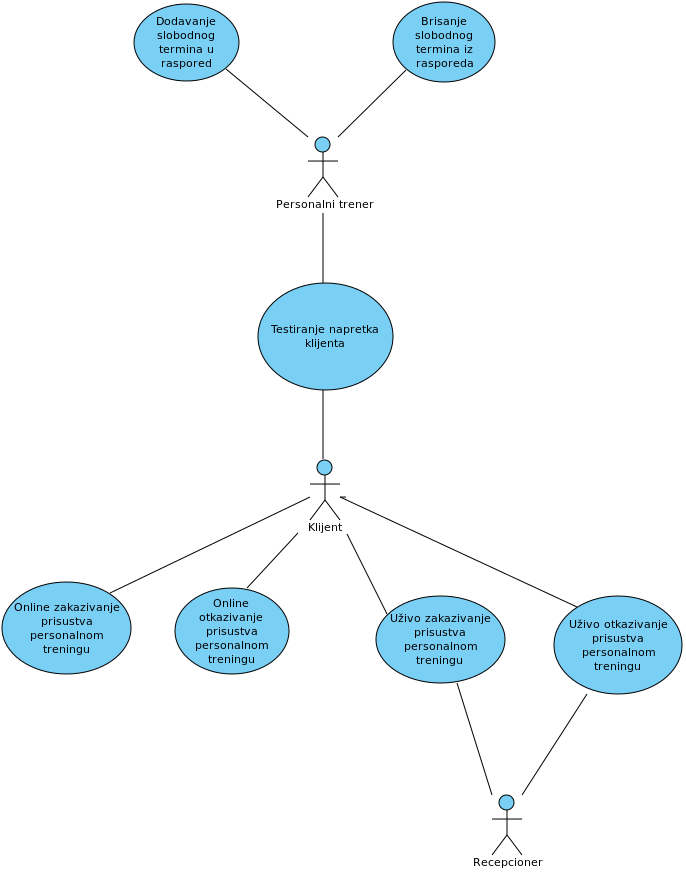
\includegraphics[scale=0.55]{sections/images/personalni_treninzi_slucajevi_upotrebe.png}
\end{center}
\caption{Dijagram slučajeva upotrebe za aktivnosti vezane za personalne treninge}
\label{fig:kontekst}
\end{figure}

\newpage

\subsubsection{Slučaj upotrebe: Dodavanje slobodnog termina u raspored}
\begin{longtable}{| p{.20\textwidth} | p{.80\textwidth} |} 
\hline
    Kratak opis &  Personalni trener vrši dodavanje slobodnog termina u svoj raspored treninga preko lične stranice na sistemu.\\ 
\hline    
    Učesnici &
    \begin{enumerate}
        \item Personalni trener - želi da doda novi slobodan termin u svoj raspored treninga
    \end{enumerate}\\
\hline
   Preduslovi & 
   \begin{enumerate}
        \item Personalni trener ima pristup internetu
        \item Personalni trener ima svoj nalog na sistemu
    \end{enumerate}\\
\hline  
    Postuslovi &
    \begin{enumerate}
        \item Termin je dodat i izmenjen je lični raspored personalnog trenera
    \end{enumerate}\\
\hline
    Osnovni tok & 
    \begin{enumerate}
        \item Personalni trener se prijavljuje na sistem
        \item Personalni trener odlazi na svoju stranicu na sistemu.
        \item Personalni trener pristupa delu stranice u kom se nalazi njegov raspored treninga.
        \item Personalni trener dodaje novu stavku u svoj raspored tako što unosi dan, sat početka i sat završetka treninga, kao i lokaciju na kojoj se trening održava.
        \item Sistem čuva informaciju o izboru i ažurira lični raspored personalnog trenera.
    \end{enumerate}\\
\hline
    Alternativni tokovi & /\\
\hline
    Podtokovi & /\\
\hline
    Specijalni zahtevi & /\\
\hline
    Dodatne informacije & /\\
\hline
\caption{Dodavanje slobodnog termina u raspored} % needs to go inside longtable environment    
\end{longtable}

\subsubsection{Slučaj upotrebe: Brisanje slobodnog termina iz rasporeda}

\begin{longtable}{| p{.20\textwidth} | p{.80\textwidth} |} 
\hline
    Kratak opis & Personalni trener vrši brisanje slobodnog termina iz svog rasporeda. \\ 
\hline    
    Učesnici &
    \begin{enumerate}
    \item  Personalni trener - želi da doda ukloni slobodan termin iz svog rasporeda treninga. 
    \end{enumerate}\\
\hline
   Preduslovi & \begin{enumerate}
    \item Personalni trener ima pristup internetu
    \item Personalni trener ima svoj nalog na sistemu
    \item Personalni trener ima slobodne termine u svom rasporedu
    \end{enumerate} \\
\hline  
    Postuslovi & 
    \begin{enumerate}
    \item Termin je izbrisan i izmenjen je lični raspored personalnog trenera
    \end{enumerate}\\
\hline
    Osnovni tok & 
    \begin{enumerate}
    \item Personalni trener se prijavljuje na sistem
    \item Personalni trener odlazi na svoju stranicu na sistemu
    \item Personalni trener pristupa delu stranice u kom se nalazi njegov raspored treninga
    \item Personalni trener briše slobodan termin tako što bira opciju 'Ukloni' koja se nalazi pored datog slobodnog termina
    \item Sistem čuva informaciju o brisanju i ažurira lični raspored personalnog trenera
    \end{enumerate}\\
\hline
    Alternativni tokovi & /\\
\hline
    Podtokovi & /\\
\hline
    Specijalni zahtevi & /\\
\hline
    Dodatne informacije & /\\
\hline
\caption{Brisanje slobodnog termina iz rasporeda}
\end{longtable}


\subsubsection{Slučaj upotrebe: Online zakazivanje prisustva personalnom treningu}

\begin{longtable}{| p{.20\textwidth} | p{.80\textwidth} |} 
\hline
    Kratak opis & Klijent zakazuje prisustvo personalnom treningu tako što bira personalnog trenera na čiji trening želi da ode, a zatim i jedan od ponuđenih slobodnih termina iz rasporeda tog trenera. \\ 
\hline    
    Učesnici & 
    \begin{enumerate}
    \item  Klijent - želi da zakaže prisustvo personalnom treningu
    \end{enumerate}\\
\hline
   Preduslovi & 
   \begin{enumerate}
    \item Klijent ima pristup internetu
    \item Klijent je registrovan
    \item Klijent je prijavljen na sistem
   \end{enumerate} \\
\hline  
    Postuslovi & 
    \begin{enumerate}
    \item Izmenjen je lični raspored personalnog trenera
    \item Izmenjen je lični raspored klijenta
   \end{enumerate} \\
\hline
    Osnovni tok &
    \begin{enumerate}
    \item Klijent odlazi na stranicu na kojoj je spisak svih personalnih trenera.
    \item Odatle, klijent pristupa stranici personalnog trenera kod koga želi da trenira.
    \item Klijent pristupa rasporedu treninga tog trenera i informiše se o slobodnim terminima. 
    
    %\textit{Koraci 1-3 se ponavljaju sve dok klijent ne pronađe slobodan termin koji mu odgovara ili dok ne pregleda rasporede svih personalnih trenera.}
    \item Klijent bira jedan od ponuđenih slobodnih termina iz rasporeda tako što klikne na opciju 'Zakaži' koja se nalazi pored svakog slobodnog termina.
    \item Sistem paralelno ažurira lične rasporede personalnog trenera (tako što unosi ime i prezime klijenta) i klijenta (tako što u odgovarajuće polje unosi naziv treninga i ime i prezime trenera).
    \item Sistem obaveštava klijenta da je uspešno zakazano prisustvo treningu.
    \item Sistem obaveštava personalnog trenera da je zakazano prisustvo jednom njegovom treningu.
   \end{enumerate} \\
\hline
    Alternativni tokovi & 
    \begin{itemize}
    \item[A3.1] Nema slobodnih termina. Ukoliko u koraku 3 nema slobodnih termina u rasporedu treninga odabranog trenera, klijent može da bira drugog trenera. Slučaj upotrebe se vraća na korak 1.
    \item[A3.2] Klijentu ne odgovaraju slobodni termini. Ukoliko u koraku 3 ima slobodnih termina u rasporedu treninga odabranog trenera, ali klijentu ne odgovara nijedan, klijent bira drugog trenera. Slučaj upotrebe se vraća na korak 1.
    \item[A3.3] Klijentu ne odgovara nijedan slobodan termin nijednog personalnog trenera. Ukoliko ponavljanjem koraka  1-3 klijent ne pronađe termin koji mu odgovara, onda neće zakazati prisustvo nijednom personalnom treningu te nedelje. Slučaj upotrebe se završava.
   \end{itemize} \\
\hline
    Podtokovi & /\\
\hline
    Specijalni zahtevi & /\\
\hline
    Dodatne informacije & / \\
\hline
\caption{ Online zakazivanje prisustva personalnom treningu}
\end{longtable}


\newpage
\begin{figure}[!ht]
\begin{center}
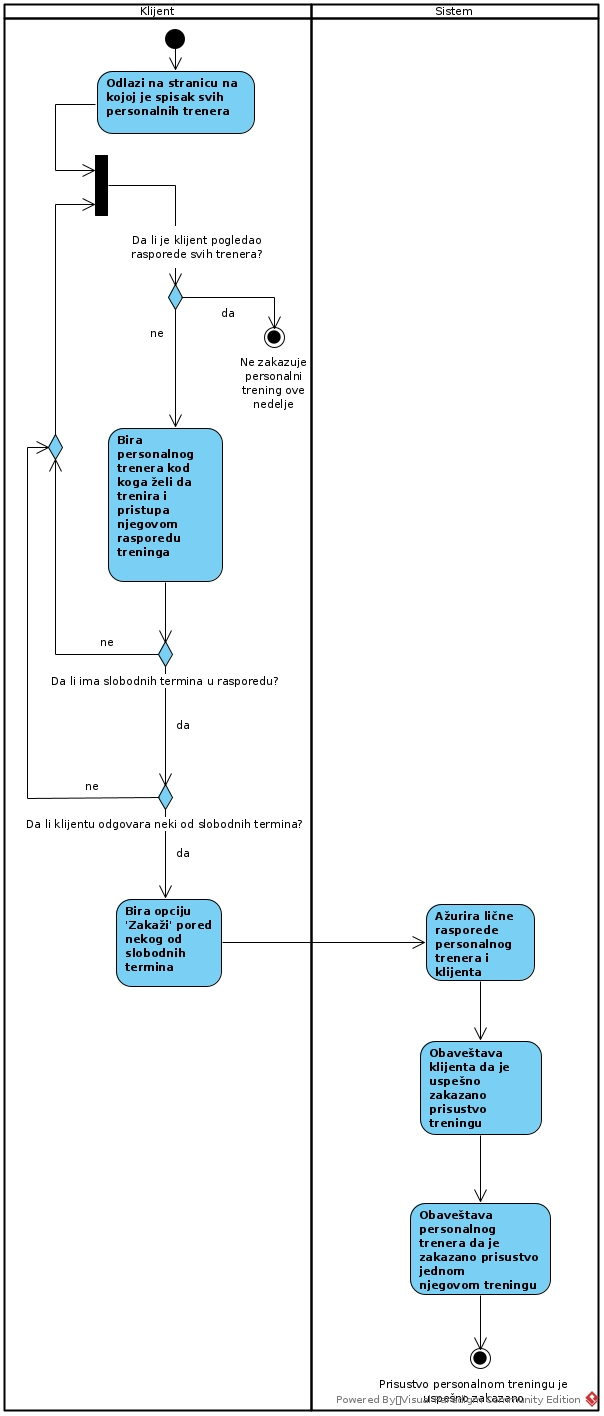
\includegraphics[scale=0.38]{sections/images/dijagram-aktivnosti-personalni-online-zakazivanje-prisustva.jpg}
\end{center}
\caption{Dijagram aktivnosti online zakazivanja prisustva personalnom treningu}
\label{fig:kontekst}
\end{figure}



\subsubsection{Slučaj upotrebe: Online otkazivanje prisustva personalnom treningu}


\begin{longtable}{| p{.20\textwidth} | p{.80\textwidth} |} 
\hline
    Kratak opis & Klijent otakazuje prisustvo prethodno prijavljenom personalnom treningu \\ 
\hline    
    Učesnici &  
    \begin{enumerate}
    \item Klijent - želi da otkaže prisustvo personalnom treningu
    \end{enumerate}\\
\hline
   Preduslovi & 
   \begin{enumerate}
    \item Klijent ima pristup internetu.
    \item Klijent je registrovan.
    \item Klijent je prijavljen na sistem.
    \item Klijent ima prijavljeno prisustvo bar jednom personalnom treningu.
   \end{enumerate}\\
\hline  
    Postuslovi & 
    \begin{enumerate}
    \item Izmenjen je lični raspored personalnog trenera.
    \item Izmenjen je lični raspored klijenta.
   \end{enumerate} \\
\hline
    Osnovni tok & 
    \begin{enumerate}
    \item Klijent odlazi na stranicu koja sadrži njegov lični raspored.
    \item Klijent bira opciju 'Otkaži' pored onog treninga kom više ne želi da prisustvuje.
    \item Sistem paralelno ažurira lični raspored klijenta (tako što iz njega uklanja taj trening) i lični raspored personalnog trenera koji drži taj trening (tako što uklanja ime i prezime korisnika čime dati termin postaje slobodan).
    \item Sistem obaveštava klijenta da je uspešno otkazano prisustvo treningu.
   \end{enumerate}\\
\hline
    Alternativni tokovi & /\\
\hline
    Podtokovi & /\\
\hline
    Specijalni zahtevi & /\\
\hline
    Dodatne informacije & /\\
\hline
\caption{Online otkazivanje prisustva personalnom treningu}
\end{longtable}




\subsubsection{Slučaj upotrebe: Uživo zakazivanje prisustva personalnom treningu}

\begin{longtable}{| p{.20\textwidth} | p{.80\textwidth} |} 
\hline
    Kratak opis & Klijent zakazuje prisustvo personalnom treningu na recepciji. \\ 
\hline    
    Učesnici & 
    \begin{enumerate}
    \item Recepcioner - prijavljuje klijenta za željeni trening
   \end{enumerate}\\
\hline
   Preduslovi & \begin{enumerate}
    \item Sistem je u funkciji.
    \item Recepcioner je prijavljen na sistem.
    \item Klijent je registrovan.
    \item Klijent razgovora uživo sa recepcionarem.
   \end{enumerate} \\
\hline  
    Postuslovi & \begin{enumerate}
    \item Klijent je dobio potvrdu da je njegov trening zakazan.
    \item Izmenjen je lični raspored personalnog trenera.
    \item Izmenjen je lični raspored klijenta.
   \end{enumerate} \\
\hline
    Osnovni tok & 
    \begin{enumerate}
    \item Klijent dolazi na recepciju sportskog centra sa ciljem da zakaže prisustvo personalnom treningu.
    \item Recepcionar traži od korisnika da mu da člansku kartu, username ili ime i prezime.
    \item Klijent daje recepcionaru svoju člansku kartu, username ili ime i prezime.
    %\item Recepcioner bira opciju zakazivanja personalnog treninga.
    \item Recepcioner pristupa delu sistema preko kog može da zakaže prisustvo treningu.
    \item Recepcioner pronalazi klijenta na osnovu nekog od datih podataka.
    \item Klijent bira trenera na čiji trening želi da se prijavi.
    \item Recepcioner proverava raspored tog trenera i govori klijentu slobodne termine.
    \item Klijent bira termin koji mu odgovara.
    \item Recepcioner vrši odabir tog termina u sistemu.
    \item Recepcioner bira opciju ``Zakaži trening``.
    \item Sistem paralelno ažurira lične rasporede klijenta i trenera.
    \item Sistem obaveštava recepcionera da je zakazano prisustvo treningu.
    \item Recepcioner obaveštava klijenta da je zakazano prisustvo treningu.
    \item Sistem obaveštava trenera da je zakazano prisustvo jednom njegovom treningu.
   \end{enumerate}\\
\hline
    Alternativni tokovi & 
    \begin{itemize}
    \item[A7.1] Nema slobodnih termina. Ukoliko u koraku 6 nema slobodnih termina u rasporedu treninga odabranog trenera, recepcioner obaveštava korisnika o tome i govori mu da izabere drugog trenera. Slučaj upotrebe se vraća na korak 5.
    \item[A7.2] Klijentu ne odgovaraju slobodni termini. Ukoliko u koraku 6 ima slobodnih termina u rasporedu treninga odabranog trenera, ali klijentu ne odgovara nijedan, klijent govori recepcioneru da mu ne odgovara nijedan ponuđeni termin i da želi da izabere drugog trenera. Slučaj upotrebe se vraća na korak 5.
    \item[A7.3] Klijentu ne odgovara nijedan slobodan termin nijednog personalnog trenera. Ukoliko ponavljanjem koraka 6 i 7 klijent ne pronađe termin koji mu odgovara, onda neće zakazati prisustvo nijednom treningu te nedelje. Slučaj upotrebe se završava.
   \end{itemize}\\
\hline
    Podtokovi & /\\
\hline
    Specijalni zahtevi & /\\
\hline
    Dodatne informacije & /\\
\hline
\caption{Uživo zakazivanje prisustva personalnom treningu}
\end{longtable}

\newpage
\begin{figure}[!ht]
\begin{center}
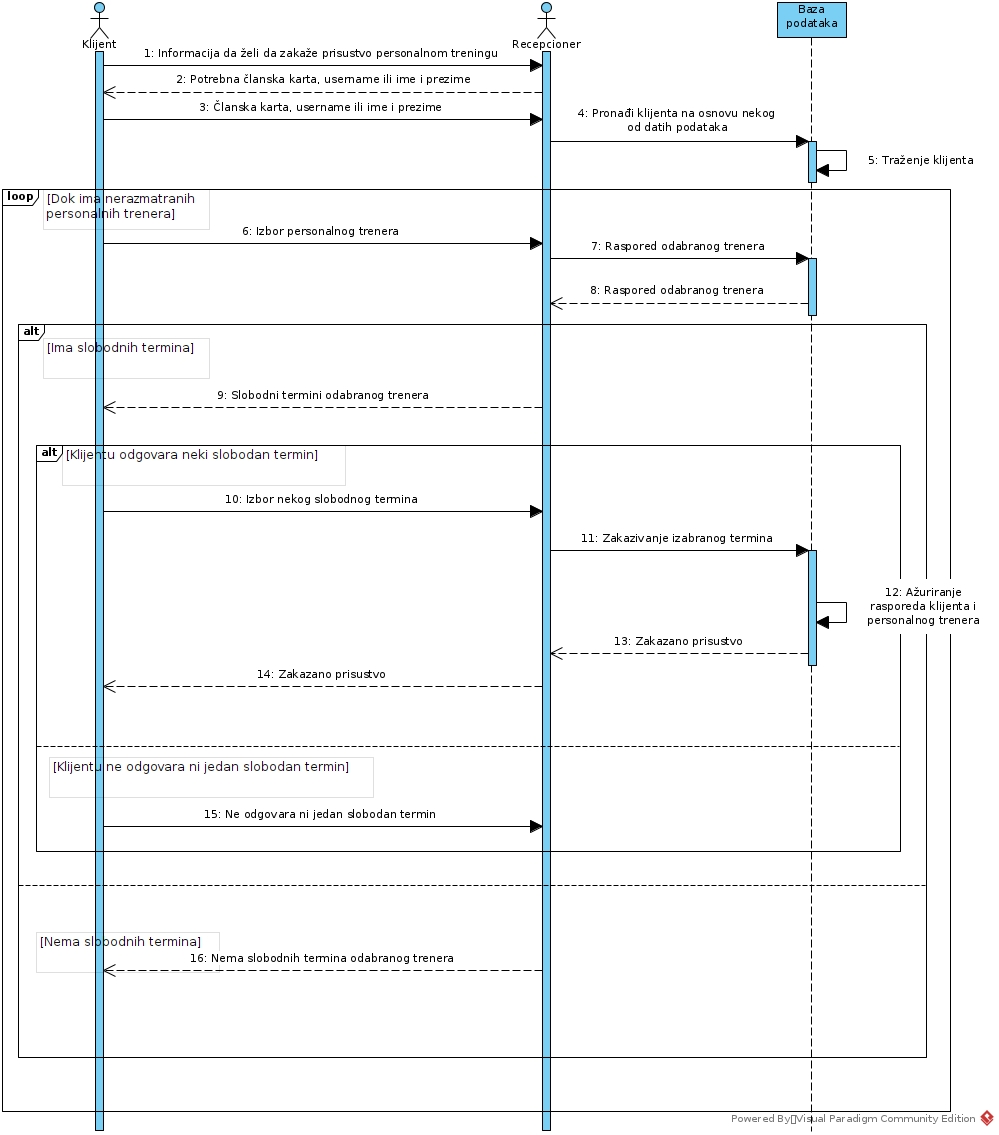
\includegraphics[scale=0.40]{sections/images/dijagram_sekvenci_personalni_uzivo_zakazivanje_prisustva.jpg}
\end{center}
\caption{Dijagram sekvenci za uživo zakazivanje prisustva personalnom treningu}
\label{fig:kontekst}
\end{figure}

    
   



\subsubsection{Slučaj upotrebe: Uživo otkazivanje prisustva personalnom treningu}

\begin{longtable}{| p{.20\textwidth} | p{.80\textwidth} |} 
\hline
    Kratak opis & Klijent otkazuje prisustvo prethodno prijavljenom personalnom treningu na recepciji. \\ 
\hline    
    Učesnici &
    \begin{enumerate}
    \item Recepcioner - odjavljuje klijenta sa odabranog treninga
   \end{enumerate}\\
\hline
   Preduslovi & \begin{enumerate}
    \item Sistem je u funkciji.
    \item Recepcioner je prijavljen na sistem.
    \item Klijent je registrovan.
    \item Klijent razgovora uživo sa recepcionarem.
    \item Klijent ima prijavljeno prisustvo bar jednom personalnom treningu.
   \end{enumerate} \\
\hline  
    Postuslovi &
    \begin{enumerate}
    \item Klijent je dobio potvrdu da je otkazano njegovo prisustvo treningu.
    \item Izmenjen je lični raspored personalnog trenera.
    \item Izmenjen je lični raspored klijenta.
   \end{enumerate}\\
\hline
    Osnovni tok & 
    \begin{enumerate}
    \item Klijent dolazi na recepciju sportskog centra.
    \item Recepcionar traži od korisnika da mu da člansku kartu, username ili ime i prezime.
    \item Klijent daje recepcionaru svoju člansku kartu username ili ime i prezime.
    \item Recepcionar se povezuje na deo sistema preko kojeg je u mogućnosti da ažurira korisnički nalog.
    \item Klijent mu govori koji je to trening kom ne želi da prisustvuje - daje mu ime i prezime trenera i termin treninga.
    \item Recepcioner u rasporedu klijenta pronalazi taj trening i bira opciju 'Otkaži'.
    \item Sistem paralelno ažurira lične rasporede klijenta i trenera.
    \item Sistem paralelno obaveštava recepcionera da je uspešno otkazano prisustvo treningu i personalnog trenera da je otkazano prisustvo jednom njegovom treningu i da je taj termin ponovo slobodan.
    \item Recepcioner obaveštava klijenta da je otkazano prisustvo treningu.
    \item Klijent odlazi.
   \end{enumerate}\\
\hline
    Alternativni tokovi & /\\
\hline
    Podtokovi & /\\
\hline
    Specijalni zahtevi & /\\
\hline
    Dodatne informacije & /\\
\hline
\caption{Uživo otkazivanje prisustva personalnom treningu}
\end{longtable}

\newpage
\begin{figure}[!ht]
\begin{center}
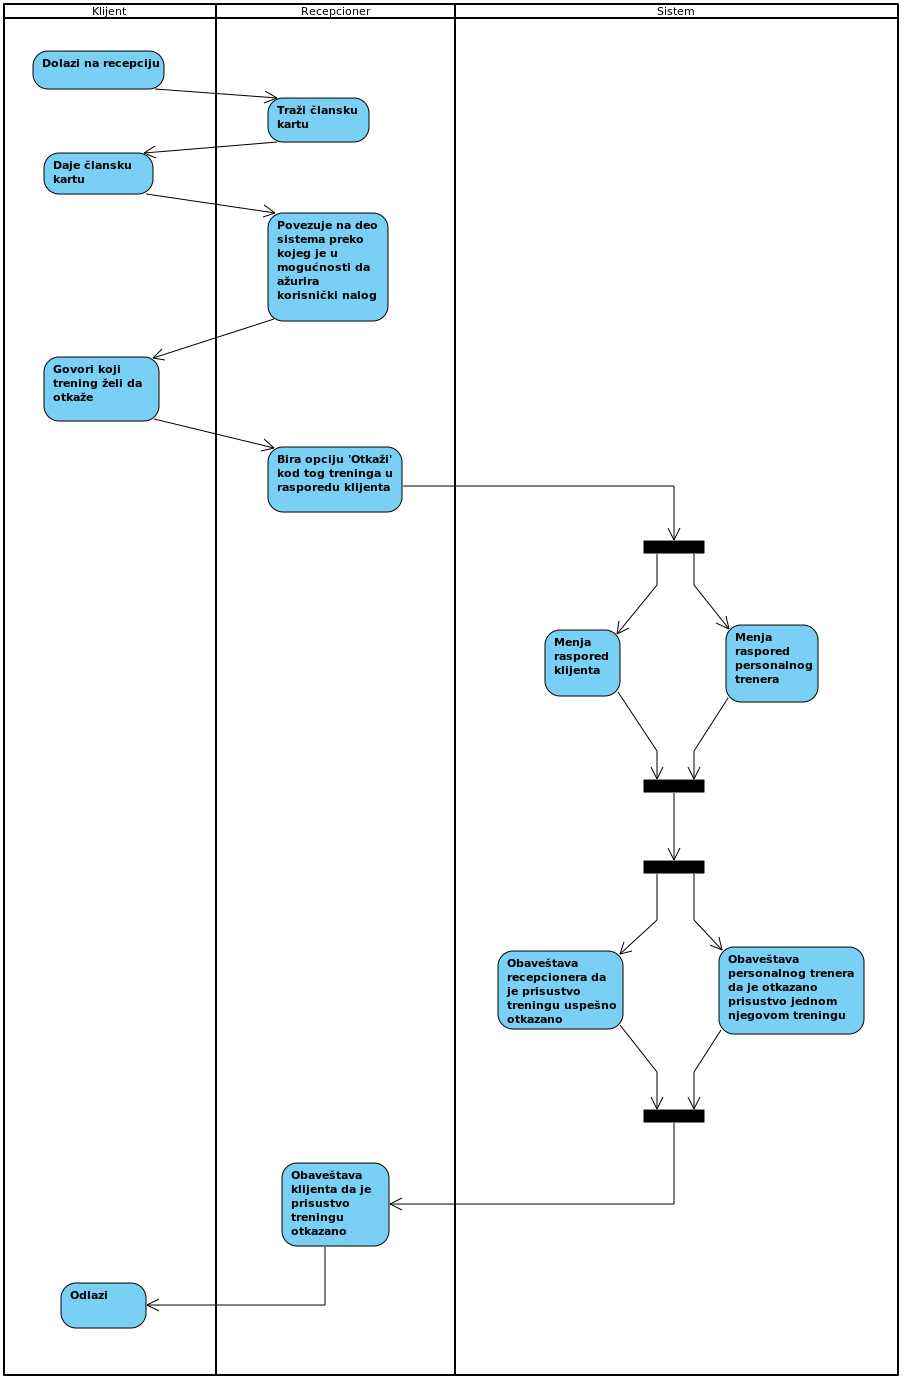
\includegraphics[scale=0.35]{sections/images/dijagram_aktivnosti_personalni_otkazivanje_uzivo.png}
\end{center}
\caption{Dijagram aktivnosti za uživo otkzivanje prisustva personalnom treningu}
\label{fig:kontekst}
\end{figure}




\subsubsection{Slučaj upotrebe: Testiranje napretka klijenta}

\begin{longtable}{| p{.20\textwidth} | p{.80\textwidth} |} 
\hline
    Kratak opis & Klijent želi da vidi koliko je napredovao korišćenjem usluga personalnih treninga i želi da dobije planove za dalje vežbanje i ishranu. \\ 
\hline    
    Učesnici & \begin{enumerate}
    \item Personalni trener
    \item Klijent
   \end{enumerate}\\
\hline
   Preduslovi & 
   \begin{enumerate}
    \item Klijent ima plaćenu članarinu za personalne treninge.
    \item Klijent i personalni trener imaju pristup internetu i prijavljeni su na sistem.
    \item Sistem je u funkciji.
   \end{enumerate}\\
\hline  
    Postuslovi &
    \begin{enumerate}
    \item Klijent je dobio nove planove vežbanja u ishrane.
    \end{enumerate}\\
\hline
    Osnovni tok & 
    \begin{enumerate}
    \item Klijent šalje poruku personalnom treneru kod koga zeli da obavi testiranje.
    \item Peronalni trener prima poruku.
    \item Klijent i personalni trener se dogovaraju o terminu testiranja.
    \item Personalni trener dodaje taj termin u svoj raspored.
    \item Klijent dodaje taj termin u svoj raspored.
    \item Sistem ažurira oba rasporeda i obaveštava učesnike da je termin uspešno dodat.
    \item Klijent i personalni terener odlaze u teretanu u dogovorenom terminu.
    \item Obavlja se niz testova kako bi se utvrdio napredak klijenta.
    \item Personalni trener smišlja nove planove treninga i ishrane i unosi ga u sistem.
    \item Sistem ažurira te planove na stranici koja je posvećena klijentu i obaveštava ga o uspešnosti akcije.
    \end{enumerate}\\
\hline
    Alternativni tokovi & \\
\hline
    Podtokovi & \\
\hline
    Specijalni zahtevi & \\
\hline
    Dodatne informacije & \\
\hline
\caption{Testiranje napretka klijenta} 
\end{longtable}